\documentclass[10.5pt]{article}
\def\examlang{en}
\def\headyear{2026--2027}
% ===== Preambul comun pentru examen, banca de probleme și setul de exerciții (XeLaTeX) =====
% Serii de timp / Time Series Analysis -- Daniel Traian Pele
% Folosire: \documentclass[10.5pt]{article}  \def\examlang{ro} (sau en)  % ===== Preambul comun pentru examen, banca de probleme și setul de exerciții (XeLaTeX) =====
% Serii de timp / Time Series Analysis -- Daniel Traian Pele
% Folosire: \documentclass[10.5pt]{article}  \def\examlang{ro} (sau en)  % ===== Preambul comun pentru examen, banca de probleme și setul de exerciții (XeLaTeX) =====
% Serii de timp / Time Series Analysis -- Daniel Traian Pele
% Folosire: \documentclass[10.5pt]{article}  \def\examlang{ro} (sau en)  \input{../tsa_exam_preamble}
% Fișierele se compilează din exam/<subfolder>/, deci logo-urile sînt în ../../logos/, iar rezultatele
% software (fișiere text generate de exam/make_figs.py) se includ cu \softout{bank/out/...} sau \softout{practice/out/...}.
\usepackage{fontspec}
\setmainfont{Helvetica Neue}
\setmonofont{Menlo}[Scale=0.92]
\usepackage{amsmath,amssymb}
\usepackage[a4paper,margin=1.9cm,top=2.4cm,headsep=0.5cm,headheight=14pt]{geometry}
\usepackage{graphicx}
\usepackage{float}
\usepackage{booktabs}
\usepackage{array}
\usepackage{enumitem}
\usepackage{xcolor}
\usepackage{fancyhdr}
\usepackage{fancyvrb}
\usepackage{lastpage}
\usepackage[hidelinks]{hyperref}
\definecolor{tsablue}{RGB}{26,58,110}
\definecolor{tsared}{RGB}{205,0,0}
\graphicspath{{../../logos/}{figs/}{../bank/figs/}{../practice/figs/}}

\providecommand{\examlang}{ro}
\newif\ifen
\def\tmpen{en}\ifx\examlang\tmpen\entrue\else\enfalse\fi

% etichete
\ifen
  \renewcommand{\figurename}{Figure}\renewcommand{\tablename}{Table}
  \newcommand{\coursetitle}{Time Series Analysis}
  \newcommand{\subjword}{Problem}
  \newcommand{\rezword}{Solution.}
  \newcommand{\baremword}{Grading:}
  \newcommand{\outword}{Software output}
\else
  \renewcommand{\figurename}{Figura}\renewcommand{\tablename}{Tabelul}
  \newcommand{\coursetitle}{Serii de timp}
  \newcommand{\subjword}{Subiectul}
  \newcommand{\rezword}{Rezolvare.}
  \newcommand{\baremword}{Barem:}
  \newcommand{\outword}{Rezultatul programului}
\fi

% comutator: barem/rezolvare (true) sau subiecte (false)
\newif\ifrez \rezfalse

% antet / subsol
\pagestyle{fancy}
\fancyhf{}
\renewcommand{\headrulewidth}{0.4pt}
\lhead{\small\itshape \coursetitle}
\providecommand{\headyear}{2027}
\rhead{\small\bfseries \headyear}
\cfoot{\small\thepage/\pageref{LastPage}}

\setlength{\parindent}{0pt}
\setlength{\parskip}{0.42ex}
\setlength{\emergencystretch}{3em}

% numerotare automată, continuă, a cerințelor (1, 2, 3, ...)
\newcounter{qq}
\newcommand{\Q}{\refstepcounter{qq}\textbf{\theqq.}~}
% punctaj aliniat la dreapta, pe ultima linie a cerinței
\newcommand{\pts}[1]{\nobreak\hfill\textnormal{\itshape (#1)}\par}

% titlu de subiect: "Subiectul I • Titlu ........ puncte" + linie
\newcommand{\subiect}[3]{%
  \vspace{1.05ex}%
  {\color{tsablue}\bfseries \subjword\ #1 \textbullet\ #2}\hfill{\bfseries #3}\par
  \vspace{0.2ex}{\color{tsablue}\hrule height0.8pt}\vspace{0.7ex}}
% subiect numerotat automat (I, II, ...); argumentul opțional = identificatorul din bancă (vizibil doar în barem)
\newcounter{subj}
\newcommand{\problem}[3][]{%
  \stepcounter{subj}%
  \subiect{\Roman{subj}}{#2\ifrez\if\relax\detokenize{#1}\relax\else\ {\normalfont\footnotesize\color{tsared}[#1]}\fi\fi}{#3}}

% rezultatul unui program (statsmodels, arch, scikit-learn), inclus dintr-un fișier text generat de make_figs.py;
% calea este relativă la exam/ (de exemplu bank/out/ch02_arma.txt)
\newcommand{\softout}[1]{\par\vspace{0.3ex}%
  \VerbatimInput[fontsize=\footnotesize,frame=lines,framesep=1.2mm,rulecolor=\color{tsablue},
    label={\footnotesize\color{tsablue}\outword}]{../#1}\par\vspace{0.2ex}}

% blocul de rezolvare (doar în barem)
\newcommand{\Rez}{\par\vspace{0.2ex}\textit{\rezword}\par\nopagebreak}
\newcommand{\barem}[1]{\par\textit{\baremword\ #1}\par}

% bloc de titlu cu sigle
\newcommand{\titlublock}[1]{%
\begin{center}
  \begin{minipage}[c]{0.16\textwidth}
\includegraphics[height=1.15cm]{ase_logo.png}\end{minipage}%
  \begin{minipage}[c]{0.68\textwidth}\centering
  \ifen
    {\bfseries Bucharest University of Economic Studies}\\[0.2ex]
    Faculty of Cybernetics, Statistics and Economic Informatics\\[0.2ex]
    Course: Time Series Analysis
  \else
    {\bfseries Academia de Studii Economice din București}\\[0.2ex]
    Facultatea de Cibernetică, Statistică și Informatică Economică\\[0.2ex]
    Disciplina: Serii de timp
  \fi
  \end{minipage}%
  \begin{minipage}[c]{0.16\textwidth}\raggedleft
\includegraphics[height=0.95cm]{ida_logo.png}\end{minipage}\\[1.2ex]
  {\large\bfseries #1}
\end{center}}

% valori utile generale (z_p, chi^2_p = cuantile de ordin p; valori critice Dickey--Fuller pentru eșantioane mari)
\newcommand{\valoriutilegen}{%
\ifen Useful values: $z_{0.975}=1.960$, $z_{0.95}=1.645$, $\chi^2_{0.95}(1)=3.84$, $\chi^2_{0.95}(2)=5.99$,
$\chi^2_{0.95}(3)=7.81$, $\chi^2_{0.95}(4)=9.49$, $\chi^2_{0.95}(5)=11.07$, $\chi^2_{0.95}(6)=12.59$,
$\chi^2_{0.95}(8)=15.51$, $\chi^2_{0.95}(10)=18.31$, $\chi^2_{0.95}(12)=21.03$, $\chi^2_{0.95}(20)=31.41$;
5\% Dickey--Fuller critical values: $-1.95$ (no constant), $-2.86$ (constant), $-3.41$ (constant and trend);
$\ln 2=0.693$ ($z_p$ and $\chi^2_p$ are quantiles of order $p$).
\else Valori utile: $z_{0,975}=1{,}960$; $z_{0,95}=1{,}645$; $\chi^2_{0,95}(1)=3{,}84$; $\chi^2_{0,95}(2)=5{,}99$;
$\chi^2_{0,95}(3)=7{,}81$; $\chi^2_{0,95}(4)=9{,}49$; $\chi^2_{0,95}(5)=11{,}07$; $\chi^2_{0,95}(6)=12{,}59$;
$\chi^2_{0,95}(8)=15{,}51$; $\chi^2_{0,95}(10)=18{,}31$; $\chi^2_{0,95}(12)=21{,}03$; $\chi^2_{0,95}(20)=31{,}41$;
valorile critice Dickey--Fuller la 5\%: $-1{,}95$ (fără constantă); $-2{,}86$ (cu constantă); $-3{,}41$ (constantă
și trend); $\ln 2=0{,}693$ ($z_p$ și $\chi^2_p$ sînt cuantile de ordin $p$).\fi}

% titlul capitolului într-un fișier din bancă (folosit doar ca etichetă de build_variant.py)
\newcommand{\banktitle}[2]{}

% Fișierele se compilează din exam/<subfolder>/, deci logo-urile sînt în ../../logos/, iar rezultatele
% software (fișiere text generate de exam/make_figs.py) se includ cu \softout{bank/out/...} sau \softout{practice/out/...}.
\usepackage{fontspec}
\setmainfont{Helvetica Neue}
\setmonofont{Menlo}[Scale=0.92]
\usepackage{amsmath,amssymb}
\usepackage[a4paper,margin=1.9cm,top=2.4cm,headsep=0.5cm,headheight=14pt]{geometry}
\usepackage{graphicx}
\usepackage{float}
\usepackage{booktabs}
\usepackage{array}
\usepackage{enumitem}
\usepackage{xcolor}
\usepackage{fancyhdr}
\usepackage{fancyvrb}
\usepackage{lastpage}
\usepackage[hidelinks]{hyperref}
\definecolor{tsablue}{RGB}{26,58,110}
\definecolor{tsared}{RGB}{205,0,0}
\graphicspath{{../../logos/}{figs/}{../bank/figs/}{../practice/figs/}}

\providecommand{\examlang}{ro}
\newif\ifen
\def\tmpen{en}\ifx\examlang\tmpen\entrue\else\enfalse\fi

% etichete
\ifen
  \renewcommand{\figurename}{Figure}\renewcommand{\tablename}{Table}
  \newcommand{\coursetitle}{Time Series Analysis}
  \newcommand{\subjword}{Problem}
  \newcommand{\rezword}{Solution.}
  \newcommand{\baremword}{Grading:}
  \newcommand{\outword}{Software output}
\else
  \renewcommand{\figurename}{Figura}\renewcommand{\tablename}{Tabelul}
  \newcommand{\coursetitle}{Serii de timp}
  \newcommand{\subjword}{Subiectul}
  \newcommand{\rezword}{Rezolvare.}
  \newcommand{\baremword}{Barem:}
  \newcommand{\outword}{Rezultatul programului}
\fi

% comutator: barem/rezolvare (true) sau subiecte (false)
\newif\ifrez \rezfalse

% antet / subsol
\pagestyle{fancy}
\fancyhf{}
\renewcommand{\headrulewidth}{0.4pt}
\lhead{\small\itshape \coursetitle}
\providecommand{\headyear}{2027}
\rhead{\small\bfseries \headyear}
\cfoot{\small\thepage/\pageref{LastPage}}

\setlength{\parindent}{0pt}
\setlength{\parskip}{0.42ex}
\setlength{\emergencystretch}{3em}

% numerotare automată, continuă, a cerințelor (1, 2, 3, ...)
\newcounter{qq}
\newcommand{\Q}{\refstepcounter{qq}\textbf{\theqq.}~}
% punctaj aliniat la dreapta, pe ultima linie a cerinței
\newcommand{\pts}[1]{\nobreak\hfill\textnormal{\itshape (#1)}\par}

% titlu de subiect: "Subiectul I • Titlu ........ puncte" + linie
\newcommand{\subiect}[3]{%
  \vspace{1.05ex}%
  {\color{tsablue}\bfseries \subjword\ #1 \textbullet\ #2}\hfill{\bfseries #3}\par
  \vspace{0.2ex}{\color{tsablue}\hrule height0.8pt}\vspace{0.7ex}}
% subiect numerotat automat (I, II, ...); argumentul opțional = identificatorul din bancă (vizibil doar în barem)
\newcounter{subj}
\newcommand{\problem}[3][]{%
  \stepcounter{subj}%
  \subiect{\Roman{subj}}{#2\ifrez\if\relax\detokenize{#1}\relax\else\ {\normalfont\footnotesize\color{tsared}[#1]}\fi\fi}{#3}}

% rezultatul unui program (statsmodels, arch, scikit-learn), inclus dintr-un fișier text generat de make_figs.py;
% calea este relativă la exam/ (de exemplu bank/out/ch02_arma.txt)
\newcommand{\softout}[1]{\par\vspace{0.3ex}%
  \VerbatimInput[fontsize=\footnotesize,frame=lines,framesep=1.2mm,rulecolor=\color{tsablue},
    label={\footnotesize\color{tsablue}\outword}]{../#1}\par\vspace{0.2ex}}

% blocul de rezolvare (doar în barem)
\newcommand{\Rez}{\par\vspace{0.2ex}\textit{\rezword}\par\nopagebreak}
\newcommand{\barem}[1]{\par\textit{\baremword\ #1}\par}

% bloc de titlu cu sigle
\newcommand{\titlublock}[1]{%
\begin{center}
  \begin{minipage}[c]{0.16\textwidth}
\includegraphics[height=1.15cm]{ase_logo.png}\end{minipage}%
  \begin{minipage}[c]{0.68\textwidth}\centering
  \ifen
    {\bfseries Bucharest University of Economic Studies}\\[0.2ex]
    Faculty of Cybernetics, Statistics and Economic Informatics\\[0.2ex]
    Course: Time Series Analysis
  \else
    {\bfseries Academia de Studii Economice din București}\\[0.2ex]
    Facultatea de Cibernetică, Statistică și Informatică Economică\\[0.2ex]
    Disciplina: Serii de timp
  \fi
  \end{minipage}%
  \begin{minipage}[c]{0.16\textwidth}\raggedleft
\includegraphics[height=0.95cm]{ida_logo.png}\end{minipage}\\[1.2ex]
  {\large\bfseries #1}
\end{center}}

% valori utile generale (z_p, chi^2_p = cuantile de ordin p; valori critice Dickey--Fuller pentru eșantioane mari)
\newcommand{\valoriutilegen}{%
\ifen Useful values: $z_{0.975}=1.960$, $z_{0.95}=1.645$, $\chi^2_{0.95}(1)=3.84$, $\chi^2_{0.95}(2)=5.99$,
$\chi^2_{0.95}(3)=7.81$, $\chi^2_{0.95}(4)=9.49$, $\chi^2_{0.95}(5)=11.07$, $\chi^2_{0.95}(6)=12.59$,
$\chi^2_{0.95}(8)=15.51$, $\chi^2_{0.95}(10)=18.31$, $\chi^2_{0.95}(12)=21.03$, $\chi^2_{0.95}(20)=31.41$;
5\% Dickey--Fuller critical values: $-1.95$ (no constant), $-2.86$ (constant), $-3.41$ (constant and trend);
$\ln 2=0.693$ ($z_p$ and $\chi^2_p$ are quantiles of order $p$).
\else Valori utile: $z_{0,975}=1{,}960$; $z_{0,95}=1{,}645$; $\chi^2_{0,95}(1)=3{,}84$; $\chi^2_{0,95}(2)=5{,}99$;
$\chi^2_{0,95}(3)=7{,}81$; $\chi^2_{0,95}(4)=9{,}49$; $\chi^2_{0,95}(5)=11{,}07$; $\chi^2_{0,95}(6)=12{,}59$;
$\chi^2_{0,95}(8)=15{,}51$; $\chi^2_{0,95}(10)=18{,}31$; $\chi^2_{0,95}(12)=21{,}03$; $\chi^2_{0,95}(20)=31{,}41$;
valorile critice Dickey--Fuller la 5\%: $-1{,}95$ (fără constantă); $-2{,}86$ (cu constantă); $-3{,}41$ (constantă
și trend); $\ln 2=0{,}693$ ($z_p$ și $\chi^2_p$ sînt cuantile de ordin $p$).\fi}

% titlul capitolului într-un fișier din bancă (folosit doar ca etichetă de build_variant.py)
\newcommand{\banktitle}[2]{}

% Fișierele se compilează din exam/<subfolder>/, deci logo-urile sînt în ../../logos/, iar rezultatele
% software (fișiere text generate de exam/make_figs.py) se includ cu \softout{bank/out/...} sau \softout{practice/out/...}.
\usepackage{fontspec}
\setmainfont{Helvetica Neue}
\setmonofont{Menlo}[Scale=0.92]
\usepackage{amsmath,amssymb}
\usepackage[a4paper,margin=1.9cm,top=2.4cm,headsep=0.5cm,headheight=14pt]{geometry}
\usepackage{graphicx}
\usepackage{float}
\usepackage{booktabs}
\usepackage{array}
\usepackage{enumitem}
\usepackage{xcolor}
\usepackage{fancyhdr}
\usepackage{fancyvrb}
\usepackage{lastpage}
\usepackage[hidelinks]{hyperref}
\definecolor{tsablue}{RGB}{26,58,110}
\definecolor{tsared}{RGB}{205,0,0}
\graphicspath{{../../logos/}{figs/}{../bank/figs/}{../practice/figs/}}

\providecommand{\examlang}{ro}
\newif\ifen
\def\tmpen{en}\ifx\examlang\tmpen\entrue\else\enfalse\fi

% etichete
\ifen
  \renewcommand{\figurename}{Figure}\renewcommand{\tablename}{Table}
  \newcommand{\coursetitle}{Time Series Analysis}
  \newcommand{\subjword}{Problem}
  \newcommand{\rezword}{Solution.}
  \newcommand{\baremword}{Grading:}
  \newcommand{\outword}{Software output}
\else
  \renewcommand{\figurename}{Figura}\renewcommand{\tablename}{Tabelul}
  \newcommand{\coursetitle}{Serii de timp}
  \newcommand{\subjword}{Subiectul}
  \newcommand{\rezword}{Rezolvare.}
  \newcommand{\baremword}{Barem:}
  \newcommand{\outword}{Rezultatul programului}
\fi

% comutator: barem/rezolvare (true) sau subiecte (false)
\newif\ifrez \rezfalse

% antet / subsol
\pagestyle{fancy}
\fancyhf{}
\renewcommand{\headrulewidth}{0.4pt}
\lhead{\small\itshape \coursetitle}
\providecommand{\headyear}{2027}
\rhead{\small\bfseries \headyear}
\cfoot{\small\thepage/\pageref{LastPage}}

\setlength{\parindent}{0pt}
\setlength{\parskip}{0.42ex}
\setlength{\emergencystretch}{3em}

% numerotare automată, continuă, a cerințelor (1, 2, 3, ...)
\newcounter{qq}
\newcommand{\Q}{\refstepcounter{qq}\textbf{\theqq.}~}
% punctaj aliniat la dreapta, pe ultima linie a cerinței
\newcommand{\pts}[1]{\nobreak\hfill\textnormal{\itshape (#1)}\par}

% titlu de subiect: "Subiectul I • Titlu ........ puncte" + linie
\newcommand{\subiect}[3]{%
  \vspace{1.05ex}%
  {\color{tsablue}\bfseries \subjword\ #1 \textbullet\ #2}\hfill{\bfseries #3}\par
  \vspace{0.2ex}{\color{tsablue}\hrule height0.8pt}\vspace{0.7ex}}
% subiect numerotat automat (I, II, ...); argumentul opțional = identificatorul din bancă (vizibil doar în barem)
\newcounter{subj}
\newcommand{\problem}[3][]{%
  \stepcounter{subj}%
  \subiect{\Roman{subj}}{#2\ifrez\if\relax\detokenize{#1}\relax\else\ {\normalfont\footnotesize\color{tsared}[#1]}\fi\fi}{#3}}

% rezultatul unui program (statsmodels, arch, scikit-learn), inclus dintr-un fișier text generat de make_figs.py;
% calea este relativă la exam/ (de exemplu bank/out/ch02_arma.txt)
\newcommand{\softout}[1]{\par\vspace{0.3ex}%
  \VerbatimInput[fontsize=\footnotesize,frame=lines,framesep=1.2mm,rulecolor=\color{tsablue},
    label={\footnotesize\color{tsablue}\outword}]{../#1}\par\vspace{0.2ex}}

% blocul de rezolvare (doar în barem)
\newcommand{\Rez}{\par\vspace{0.2ex}\textit{\rezword}\par\nopagebreak}
\newcommand{\barem}[1]{\par\textit{\baremword\ #1}\par}

% bloc de titlu cu sigle
\newcommand{\titlublock}[1]{%
\begin{center}
  \begin{minipage}[c]{0.16\textwidth}
\includegraphics[height=1.15cm]{ase_logo.png}\end{minipage}%
  \begin{minipage}[c]{0.68\textwidth}\centering
  \ifen
    {\bfseries Bucharest University of Economic Studies}\\[0.2ex]
    Faculty of Cybernetics, Statistics and Economic Informatics\\[0.2ex]
    Course: Time Series Analysis
  \else
    {\bfseries Academia de Studii Economice din București}\\[0.2ex]
    Facultatea de Cibernetică, Statistică și Informatică Economică\\[0.2ex]
    Disciplina: Serii de timp
  \fi
  \end{minipage}%
  \begin{minipage}[c]{0.16\textwidth}\raggedleft
\includegraphics[height=0.95cm]{ida_logo.png}\end{minipage}\\[1.2ex]
  {\large\bfseries #1}
\end{center}}

% valori utile generale (z_p, chi^2_p = cuantile de ordin p; valori critice Dickey--Fuller pentru eșantioane mari)
\newcommand{\valoriutilegen}{%
\ifen Useful values: $z_{0.975}=1.960$, $z_{0.95}=1.645$, $\chi^2_{0.95}(1)=3.84$, $\chi^2_{0.95}(2)=5.99$,
$\chi^2_{0.95}(3)=7.81$, $\chi^2_{0.95}(4)=9.49$, $\chi^2_{0.95}(5)=11.07$, $\chi^2_{0.95}(6)=12.59$,
$\chi^2_{0.95}(8)=15.51$, $\chi^2_{0.95}(10)=18.31$, $\chi^2_{0.95}(12)=21.03$, $\chi^2_{0.95}(20)=31.41$;
5\% Dickey--Fuller critical values: $-1.95$ (no constant), $-2.86$ (constant), $-3.41$ (constant and trend);
$\ln 2=0.693$ ($z_p$ and $\chi^2_p$ are quantiles of order $p$).
\else Valori utile: $z_{0,975}=1{,}960$; $z_{0,95}=1{,}645$; $\chi^2_{0,95}(1)=3{,}84$; $\chi^2_{0,95}(2)=5{,}99$;
$\chi^2_{0,95}(3)=7{,}81$; $\chi^2_{0,95}(4)=9{,}49$; $\chi^2_{0,95}(5)=11{,}07$; $\chi^2_{0,95}(6)=12{,}59$;
$\chi^2_{0,95}(8)=15{,}51$; $\chi^2_{0,95}(10)=18{,}31$; $\chi^2_{0,95}(12)=21{,}03$; $\chi^2_{0,95}(20)=31{,}41$;
valorile critice Dickey--Fuller la 5\%: $-1{,}95$ (fără constantă); $-2{,}86$ (cu constantă); $-3{,}41$ (constantă
și trend); $\ln 2=0{,}693$ ($z_p$ și $\chi^2_p$ sînt cuantile de ordin $p$).\fi}

% titlul capitolului într-un fișier din bancă (folosit doar ca etichetă de build_variant.py)
\newcommand{\banktitle}[2]{}

\renewcommand{\subjword}{Problem}
\newcommand{\pp}[1]{\stepcounter{subj}\subiect{\arabic{subj}}{#1}{}}
\newcommand{\capitol}[1]{\par\vspace{1.4ex}{\large\bfseries\color{tsared}#1}\par\vspace{0.4ex}}
\setlist[enumerate]{label=(\alph*),leftmargin=2.2em,itemsep=0.15ex,topsep=0.3ex}
\begin{document}
\titlublock{EXAM PROBLEMS --- PRACTICE SET}

\noindent The problems have the form of exam problems: the interpretation of a software output, a short derivation
or the choice of a model. The data are the series used in the course (last day: 18 September 2026), and the software
outputs (\texttt{statsmodels}, \texttt{arch}, \texttt{scikit-learn}) are shown as the programs print them. The
numerical answers are at the end of the document.
Notation: $\varepsilon_t$ white noise with variance $\sigma^2$; $L$ the lag operator; $r_t=100\ln(P_t/P_{t-1})$ the log
return in \%; $\mathrm{VaR}_\alpha=-q_\alpha$ (VaR 1\% is the loss exceeded on 1\% of the days).\par
\vspace{0.4ex}{\small\noindent\valoriutilegen\par}

% ===================================================================================================
\capitol{Chapter 1. Stochastic processes and stationarity}

\pp{The correlogram of the Nile flow}
The annual flow of the Nile at Aswan ($10^8$ m$^3$, 1871--1970, $n=100$, mean $919.4$) has the correlogram below.
\softout{practice/out/p_nile_corr.txt}
\begin{enumerate}
\item Compute the limits of the 95\% confidence band for the sample autocorrelations under the white-noise hypothesis.
\item State the decision of the Ljung--Box test with 10 lags at the 5\% significance level.
\item Identify the ARMA model suggested by the pattern of the ACF and the PACF.
\end{enumerate}

\pp{The US 10-year Treasury yield: level and change}
Figure~\ref{fig:us10y} shows the 10-year US Treasury yield (daily, 2015--2026) and its daily change in basis points.
For the level, the first five sample autocorrelations are $0.998$; $0.997$; $0.995$; $0.993$; $0.992$. For the daily
change ($n=2926$) they are $-0.037$; $-0.036$; $0.006$; $-0.012$; $-0.008$.
\begin{figure}[H]\centering
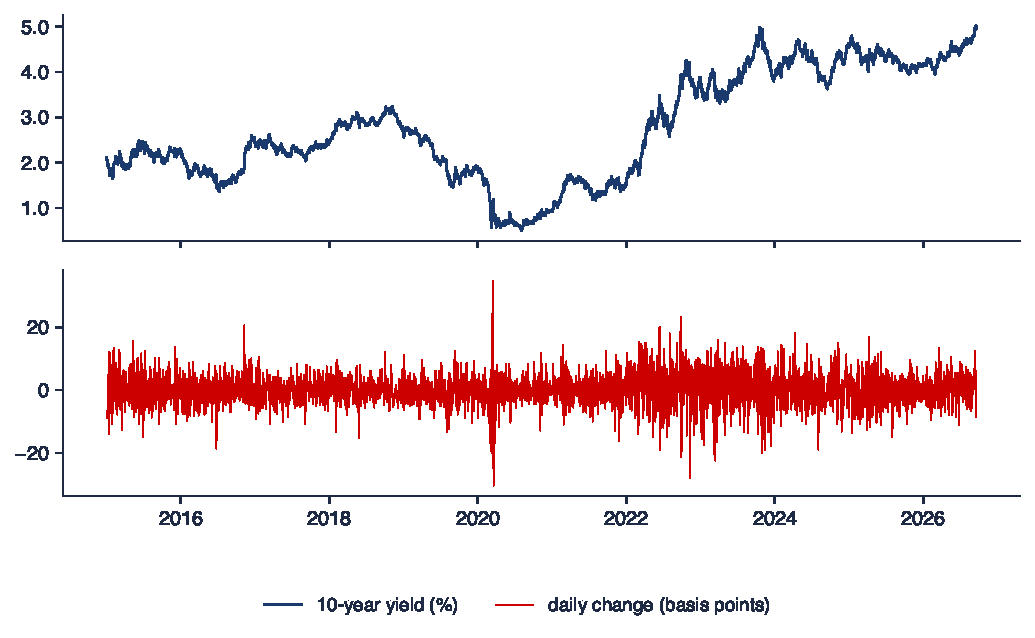
\includegraphics[width=0.66\textwidth]{practice_us10y_en.pdf}
\caption{The 10-year US Treasury yield and its daily change, 2015--2026.}\label{fig:us10y}
\end{figure}
\begin{enumerate}
\item Compute the Ljung--Box statistic $Q(5)=n(n+2)\sum_{k=1}^{5}\hat\rho_k^2/(n-k)$ for the daily change.
\item State the decision of the test at the 5\% significance level.
\item Explain why autocorrelations of the level close to 1 do not indicate a stationary series.
\end{enumerate}

\pp{A white noise that is not independent}
Let $Y_t=\varepsilon_t\varepsilon_{t-1}$, where $\varepsilon_t$ are independent $N(0,\sigma^2)$ variables, so that
$E(\varepsilon_t^4)=3\sigma^4$.
\begin{enumerate}
\item Compute the mean and the variance of $Y_t$.
\item Show that $\mathrm{Cov}(Y_t,Y_{t-k})=0$ for every $k\ge 1$.
\item Compute the correlation between $Y_t^2$ and $Y_{t-1}^2$.
\end{enumerate}

% ===================================================================================================
\capitol{Chapter 2. ARMA models}

\pp{The AR(2) model of the sunspots}
The yearly sunspot number (1700--2008) was modelled with an AR(2) with constant,
$y_t-\mu=\phi_1(y_{t-1}-\mu)+\phi_2(y_{t-2}-\mu)+\varepsilon_t$ (in \texttt{statsmodels}, \texttt{const} is the mean $\mu$).
\softout{practice/out/p_sunspots_ar2.txt}
The observed values are $y_{2007}=7.5$ and $y_{2008}=2.9$.
\begin{enumerate}
\item Check the stationarity conditions of the estimated AR(2) model.
\item Show that the roots of the autoregressive polynomial are complex.
\item Compute the period of the cycle from $\cos(2\pi/P)=\phi_1/\bigl(2\sqrt{-\phi_2}\bigr)$.
\item Compute the forecast for 2009.
\end{enumerate}

\pp{Choosing the ARMA order: US industrial production}
For the monthly growth of US industrial production, $g_t=100\,\Delta\ln \mathrm{INDPRO}_t$, six ARMA models with
constant were estimated.
\softout{practice/out/p_indpro_orders.txt}
The estimated AR(1) model is $g_t=0.116+0.202\,(g_{t-1}-0.116)+\varepsilon_t$, with $\hat\sigma^2=1.015$; in December
2025, $g_T=0.454$.
\begin{enumerate}
\item State the model chosen by the AIC and the model chosen by the BIC.
\item Interpret the column of Ljung--Box $p$-values of the residuals.
\item Compute the AR(1) forecasts for January and February 2026.
\item Compute the standard deviation of the two-step forecast error.
\end{enumerate}

\pp{The autocorrelation of an MA(1)}
Let $y_t=\varepsilon_t+\theta\varepsilon_{t-1}$.
\begin{enumerate}
\item Show that $\rho(1)=\theta/(1+\theta^2)$ and $\rho(k)=0$ for $k\ge 2$.
\item Find the values of $\theta$ for which $\rho(1)=0.4$.
\item Justify the choice of one of the two values.
\end{enumerate}

% ===================================================================================================
\capitol{Chapter 3. Unit roots and ARIMA models}

\pp{The ADF test for the gold price}
The augmented Dickey--Fuller (ADF) test was applied to the log of the monthly gold price (USD per ounce, January
2010 -- August 2026), in levels and in first differences.
\softout{practice/out/p_gold_adf.txt}
\begin{enumerate}
\item State the decision of the test for the level at the 5\% significance level.
\item State the decision of the test for the first difference.
\item State the order of integration of the series.
\item Explain the choice of the deterministic terms in the two regressions.
\end{enumerate}

\pp{An ARIMA(0,1,1) forecast with drift: gold}
For $y_t=100\ln P_t$ (the monthly gold price) the model $\Delta y_t=c+\varepsilon_t+\theta\varepsilon_{t-1}$ was
estimated.
\softout{practice/out/p_gold_ima.txt}
\begin{enumerate}
\item Test the significance of $\theta$.
\item State the simpler model suggested by the result.
\item Compute the forecasts for September and October 2026 with the estimated model.
\item Compute the standard deviations of the one-step and two-step forecast errors, given that $\psi_1=1+\theta$.
\item Convert the forecast for September 2026 into a price (USD per ounce).
\end{enumerate}

\pp{ADF and KPSS for US consumer prices}
The ADF test (null hypothesis: unit root) and the KPSS test (null hypothesis: stationarity) were applied to the US
consumer price index (CPIAUCSL, monthly, 1990--2025).
\softout{practice/out/p_cpi_tests.txt}
\begin{enumerate}
\item State the joint conclusion of the two tests for $\ln \mathrm{CPI}$.
\item State the joint conclusion for the inflation rate.
\item State the order of integration of $\ln \mathrm{CPI}$.
\end{enumerate}

% ===================================================================================================
\capitol{Chapter 4. Seasonality and forecasting}

\pp{The airline model for the CO$_2$ concentration}
The monthly CO$_2$ concentration at Mauna Loa (ppm, 1960--2000) was modelled with a SARIMA$(0,1,1)(0,1,1)_{12}$.
\softout{practice/out/p_co2_airline.txt}
\begin{enumerate}
\item Write the equation of the model with the lag operator.
\item Compute the coefficient of $\varepsilon_{t-13}$.
\item State the decision of the Ljung--Box test for the residuals ($24-2=22$ degrees of freedom;
$\chi^2_{0.95}(22)=33.92$).
\item Compute the theoretical autocorrelations $\rho(1)$ and $\rho(12)$ of the series $(1-L)(1-L^{12})y_t$.
\end{enumerate}

\pp{Forecast evaluation: tourist nights in Romania}
For the monthly number of nights spent in tourist accommodation in Romania (millions, Eurostat), the year 2025 was
forecast from December 2024 with the seasonal naive method and with a SARIMA model (Figure~\ref{fig:tour}).
\softout{practice/out/p_tourism_eval.txt}
For the differences $d_t=|e_t^{\text{naive}}|-|e_t^{\text{SARIMA}}|$ of the 12 months, the mean is $\bar d=-0.1234$ and
the standard deviation is $s_d=0.210$.
\begin{figure}[H]\centering
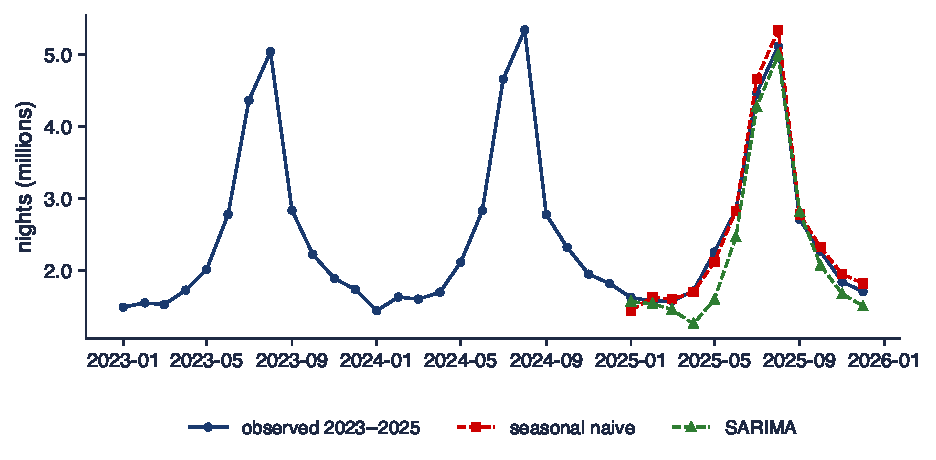
\includegraphics[width=0.66\textwidth]{practice_tourism_en.pdf}
\caption{Monthly nights in Romania and the forecasts for 2025.}\label{fig:tour}
\end{figure}
\begin{enumerate}
\item Compute the MASE of both methods.
\item Compute the Diebold--Mariano statistic $\mathrm{DM}=\bar d/(s_d/\sqrt{12})$.
\item State the decision of the Diebold--Mariano test at the 5\% significance level.
\item Explain the weak result of the SARIMA model.
\end{enumerate}

\pp{The seasonal difference}
In July and August 2024 there were $4.660$ and $5.346$ million nights, and in July and August 2025, $4.467$ and
$5.117$ million.
\begin{enumerate}
\item Compute $\Delta_{12}\ln y_t=\ln y_t-\ln y_{t-12}$ for July and August 2025, in \%.
\item Show that $1-L^{12}=(1-L)(1+L+\dots+L^{11})$.
\item Show that $\Delta_{12}$ removes a deterministic seasonal component $s_t=s_{t-12}$.
\end{enumerate}

% ===================================================================================================
\capitol{Chapter 5. Conditional volatility and GARCH models}

\pp{GARCH(1,1)-$t$ for the DAX}
For the daily log returns of the DAX index the model $\sigma_t^2=\omega+\alpha\varepsilon_{t-1}^2+\beta\sigma_{t-1}^2$
with Student-$t$ innovations was estimated.
\softout{practice/out/p_dax_garch.txt}
\begin{enumerate}
\item Compute the persistence of volatility.
\item Compute the long-run volatility, daily and annualised (252 days).
\item Compute the half-life of a volatility shock.
\item Compute the excess kurtosis of the Student-$t$ innovations, $6/(\nu-4)$.
\item Interpret the excess kurtosis of the innovations.
\end{enumerate}

\pp{One GARCH step and VaR 1\%: Ethereum}
A GARCH(1,1) with Normal innovations, estimated on the daily returns of Ethereum (2018--2026), has $\hat\mu=0.083$;
$\hat\omega=0.503$; $\hat\alpha=0.064$; $\hat\beta=0.911$. On 18 September 2026 the conditional variance was
$\sigma_T^2=10.225$ and the return was $r_T=6.496\%$. Use $z_{0.01}=-2.326$.
\begin{enumerate}
\item Compute the conditional variance for 19 September 2026.
\item Compute the VaR 1\% for 19 September 2026, in \%.
\item Compute the corresponding loss for a position of USD 10,000.
\end{enumerate}

\pp{The asymmetry of volatility: GJR-GARCH for the DAX}
On the same DAX data a GJR-GARCH(1,1,1) with Student-$t$ innovations was estimated,
$\sigma_t^2=\omega+(\alpha+\gamma I_{t-1})\varepsilon_{t-1}^2+\beta\sigma_{t-1}^2$, where $I_{t-1}=1$ if
$\varepsilon_{t-1}<0$.
\softout{practice/out/p_dax_gjr.txt}
\begin{enumerate}
\item Test the GARCH(1,1)-$t$ model against the GJR-GARCH with a likelihood ratio test.
\item Compute $\sigma_t^2$ after a shock $\varepsilon_{t-1}=-2$ and after a shock $\varepsilon_{t-1}=+2$, with
$\sigma_{t-1}^2=1$.
\item Compute the persistence $\alpha+\gamma/2+\beta$.
\item Interpret the estimate $\hat\alpha=0$.
\end{enumerate}

% ===================================================================================================
\capitol{Chapter 6. VAR models and Granger causality}

\pp{A macroeconomic VAR: United States, 1959--2009}
For the vector of real GDP growth (annualised, \%), inflation and the 3-month Treasury bill rate (quarterly data, the
\texttt{macrodata} set) the information criteria and the Granger causality tests in a VAR(2) with constant were
computed.
\softout{practice/out/p_macro_var.txt}
\begin{enumerate}
\item State the order chosen by each information criterion.
\item Compute the number of coefficients of a VAR(6) and of a VAR(1) with three variables and a constant.
\item Interpret the Granger causality test from the interest rate to GDP growth.
\item Interpret the Granger causality test from GDP growth to the interest rate.
\end{enumerate}

\pp{The stability and the forecast of a VAR(1)}
A VAR(1) for $x_t=(g_t,\Delta i_t)'$, US real GDP growth and the change in the 3-month interest rate, has the equations
\[
g_t=2.259+0.273\,g_{t-1}+0.612\,\Delta i_{t-1}+u_{1t},\qquad
\Delta i_t=-0.115+0.031\,g_{t-1}+0.006\,\Delta i_{t-1}+u_{2t}.
\]
In the third quarter of 2009, $g_T=2.74$ and $\Delta i_T=-0.06$.
\begin{enumerate}
\item Compute the eigenvalues of the coefficient matrix from its trace and determinant.
\item Compute the forecast for the fourth quarter of 2009.
\item Compute the unconditional mean of the process, $\mu=(I-A)^{-1}c$.
\end{enumerate}

% ===================================================================================================
\capitol{Chapter 7. Cointegration and VECM}

\pp{The Engle--Granger method: US 10-year and 3-month rates}
The Engle--Granger method was applied to the 10-year (GS10) and 3-month (TB3MS) US Treasury yields, monthly data
1990--2025. The 5\% Engle--Granger critical value for two variables with a constant is $-3.34$.
\softout{practice/out/p_rates_eg.txt}
\begin{enumerate}
\item Interpret the comparison between the $R^2$ and the Durbin--Watson statistic.
\item State the decision of the cointegration test at the 5\% significance level.
\item Explain why the $p$-value from the Dickey--Fuller table cannot be used in step 2.
\end{enumerate}

\pp{The Johansen test and the VECM: the term structure}
On the longer sample 1960--2025 the Johansen tests were applied and a VECM with rank 1 was estimated,
$\Delta x_t=\alpha\beta' x_{t-1}+\dots$, with $x_t=(\mathrm{GS10}_t,\mathrm{TB3MS}_t)'$.
\softout{practice/out/p_rates_vecm.txt}
In December 2025, GS10 $=4.14$ and TB3MS $=3.59$.
\begin{enumerate}
\item Determine the cointegration rank with the trace statistic.
\item Write the long-run equilibrium relation.
\item Interpret the long-run equilibrium relation.
\item Compute the half-life of a deviation from equilibrium, with $z_t=z_{t-1}(1+\alpha_1+\beta_2\alpha_2)$.
\item Compute the deviation from equilibrium in December 2025.
\item Compute the expected corrections of the two rates.
\end{enumerate}

% ===================================================================================================
\capitol{Chapter 8. Long memory and ARFIMA models}

\pp{The GPH estimator for the VIX index}
The memory parameter $d$ of the log of the VIX index (daily, 2004--2026) was estimated with the Geweke--Porter-Hudak
(GPH) log-periodogram regression.
\softout{practice/out/p_vix_gph.txt}
\begin{enumerate}
\item Compute the 95\% confidence interval for $d$ with the asymptotic standard error.
\item Test the hypothesis $d=0.5$.
\item Interpret the result of the test.
\item Check the consistency of the estimate for the series with the estimate for its first difference.
\item Compute the first three weights $\pi_k$ of $(1-L)^d$ for $d=0.63$, with $\pi_k=\pi_{k-1}(k-1-d)/k$.
\end{enumerate}

\pp{The long memory of volatility: gold}
Figure~\ref{fig:goldacf} shows the autocorrelation function of the daily absolute returns of gold (2010--2026,
$n=4350$). The sample values are $\hat\rho(1)=0.110$; $\hat\rho(10)=0.164$; $\hat\rho(100)=0.081$.
\begin{figure}[H]\centering
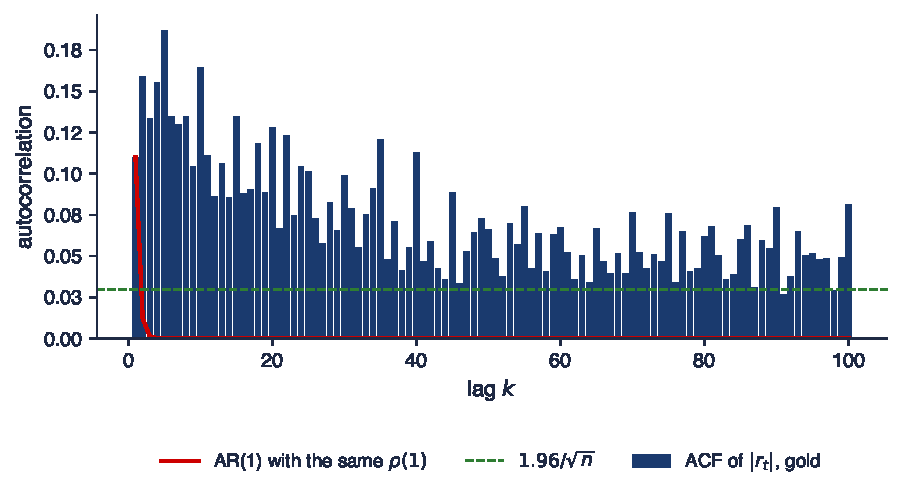
\includegraphics[width=0.64\textwidth]{practice_gold_absacf_en.pdf}
\caption{Autocorrelations of $|r_t|$ for gold and of an AR(1) with the same $\rho(1)$.}\label{fig:goldacf}
\end{figure}
\begin{enumerate}
\item Compute $\rho(10)$ and $\rho(100)$ for an AR(1) with $\rho(1)=0.110$.
\item Estimate $d$ from the slope of the power law $\rho(k)\approx Ck^{2d-1}$, using lags 10 and 100.
\item Name a suitable model for this volatility.
\end{enumerate}

% ===================================================================================================
\capitol{Chapter 9. Machine learning for time series}

\pp{The sign of the Bitcoin return}
Two classifiers forecast the sign of the next-day Bitcoin return, with five lags and the 20-day volatility as
features.
\softout{practice/out/p_btc_sign.txt}
\begin{enumerate}
\item Compute the statistic $z=(\hat a-a_0)/\sqrt{a_0(1-a_0)/n}$ for the random forest against the ``always up''
benchmark.
\item Explain why the right benchmark is the majority class and not an accuracy of 50\%.
\item Explain why cross-validation with random folds would overstate the accuracy.
\end{enumerate}

\pp{Conformal intervals and the pinball loss: gold}
For the daily return of gold the point forecast is 0, and the conformity scores are the absolute errors. The 20
calibration scores (sorted) are: $0.13$; $0.14$; $0.32$; $0.53$; $0.63$; $0.68$; $0.77$; $1.00$; $1.14$; $1.15$; $1.38$;
$1.55$; $1.66$; $1.79$; $1.81$; $2.12$; $2.14$; $2.90$; $3.01$; $4.05$. The returns of 14--18 September 2026 are $-1.39$;
$-0.12$; $-0.27$; $1.73$; $0.77$.
\begin{enumerate}
\item Compute the 90\% conformal interval, with the score of order $\lceil (n+1)(1-\alpha)\rceil$.
\item Compute the share of the returns of 14--18 September 2026 that fall inside the interval.
\item Compute the mean pinball loss, with $\tau=0.05$, of the quantile forecasts $q_A=-1.2$ and $q_B=-2.5$.
\end{enumerate}

% ===================================================================================================
\capitol{Chapter 10. State space models, the Kalman filter and Markov switching}

\pp{The Kalman filter for the US unemployment rate}
The monthly US unemployment rate (2022--2025) was modelled with a local level model, $y_t=\mu_t+\varepsilon_t$,
$\mu_{t+1}=\mu_t+\eta_t$. The value for October 2025 is missing (it was not published).
\softout{practice/out/p_unrate_ll.txt}
In January 2026 the unemployment rate was $4.3\%$.
\begin{enumerate}
\item Compute the signal-to-noise ratio $q=\sigma^2_\eta/\sigma^2_\varepsilon$.
\item Compute the prediction variance, the Kalman gain and the filtered level for January 2026.
\item Describe the filter step for the missing month (October 2025).
\end{enumerate}

\pp{Volatility regimes: Nasdaq 100}
The weekly returns of the Nasdaq 100 index (2015--2026) were modelled with a two-regime Markov switching model.
\softout{practice/out/p_ndx_ms.txt}
\begin{enumerate}
\item Compute the expected duration of each regime, $1/(1-p_{ii})$, in weeks.
\item Compute the ergodic probability of the turbulent regime.
\item Compare the ergodic probability with the observed share of turbulent weeks.
\item Compute the annualised volatility (52 weeks) of each regime.
\end{enumerate}

% ===================================================================================================
\clearpage
\capitol{Answers}
{\small
\begin{enumerate}[label=\textbf{\arabic*.},leftmargin=2.2em,itemsep=0.25ex]
\item (a) $\pm 1.96/\sqrt{100}=\pm 0.196$. (b) $Q(10)=88.13>18.31$: white noise is rejected. (c) AR(1): the ACF decays
gradually (8 of the first 10 autocorrelations are outside the band) and the PACF is significant only at lag 1
($0.498$).
\item (a) $Q(5)=8.52$. (b) $8.52<11.07$: the hypothesis of uncorrelated changes is not rejected (although
$\hat\rho_1=-0.037$ is at the edge of the band $\pm 0.036$). (c) For a random walk the sample ACF stays close to 1 over
many lags; the level does not revert to a constant mean, and differencing makes it stationary.
\item (a) $E(Y_t)=0$; $\mathrm{Var}(Y_t)=\sigma^4$. (b) Every term of the product contains an $\varepsilon$ that appears
only once, with mean 0. (c) $\mathrm{Cov}(Y_t^2,Y_{t-1}^2)=3\sigma^8-\sigma^8=2\sigma^8$;
$\mathrm{Var}(Y_t^2)=9\sigma^8-\sigma^8=8\sigma^8$; the correlation is $0.25$: white noise, but not independent.
\item (a) $\phi_1+\phi_2=0.702<1$; $\phi_2-\phi_1=-2.079<1$; $|\phi_2|=0.689<1$: stationary.
(b) $\phi_1^2+4\phi_2=-0.821<0$. (c) $\cos(2\pi/P)=0.838$; $P=10.9$ years. (d) $\hat y_{2009}=13.69$.
\item (a) AIC: ARMA(2,0); BIC: ARMA(0,1). (b) All $p$-values are below $0.05$: autocorrelation remains in the residuals
(least for the AR(2), $p=0.034$); the models are too simple. (c) $0.184$; $0.130$. (d)
$\sqrt{1.015(1+0.202^2)}=1.028$.
\item (a) $\gamma(0)=\sigma^2(1+\theta^2)$, $\gamma(1)=\theta\sigma^2$, $\gamma(k)=0$ for $k\ge 2$.
(b) $0.4\theta^2-\theta+0.4=0$: $\theta=0.5$ or $\theta=2$. (c) $\theta=0.5$, the only invertible value ($|\theta|<1$).
\item (a) $-0.407>-3.433$: the unit root is not rejected. (b) $-14.04<-2.876$: rejected. (c) $I(1)$.
(d) The level trends, hence constant and trend; the difference fluctuates around a non-zero mean, hence a constant.
\item (a) $z=-0.185$, $p=0.853$: $\theta$ is not significant. (b) A random walk with drift is enough. (c) $840.723$; $841.434$. (d) $4.667$; $6.561$. (e) $e^{8.40723}=4479.3$ USD per ounce.
\item (a) ADF does not reject the unit root ($p=0.610$), KPSS rejects stationarity ($0.260>0.146$): unit root.
(b) ADF rejects ($p=0.001$), KPSS does not reject ($0.203<0.463$): inflation is stationary. (c) $\ln\mathrm{CPI}\sim I(1)$.
\item (a) $(1-L)(1-L^{12})y_t=(1-0.352L)(1-0.858L^{12})\varepsilon_t$. (b) The coefficient of $\varepsilon_{t-13}$ is $\theta\Theta=0.302$. (c) $Q(24)=19.42<33.92$ ($p=0.619$): the residuals are white noise. (d) $\rho(1)=-0.313$; $\rho(12)=-0.494$.
\item (a) $0.617$ (seasonal naive); $1.381$ (SARIMA). (b) $\mathrm{DM}=-2.04$. (c) $|-2.04|>1.96$: equal accuracy is
rejected; the seasonal naive method is better. (d) The model strongly underestimates the spring (April: $1.256$
against $1.716$; May: $1.595$ against $2.256$): estimated on 2015--2024, with the pandemic years, it misses the level
reached after 2022, which the seasonal naive method takes directly from 2024.
\item (a) July: $-4.23\%$; August: $-4.38\%$. (b) The product telescopes: $(1-L)\sum_{j=0}^{11}L^j=1-L^{12}$.
(c) $(1-L^{12})s_t=s_t-s_{t-12}=0$.
\item (a) $\alpha+\beta=0.9815$. (b) $\bar\sigma^2=0.0364/0.0185=1.968$; $1.403\%$ per day; $22.27\%$ per year. (c) $\ln 0.5/\ln 0.9815=37.1$ days. (d) $6/1.468=4.09$. (e) Fat tails; the kurtosis is finite because $\nu>4$.
\item (a) $0.503+0.064\cdot 6.413^2+0.911\cdot 10.225=12.45$ ($\varepsilon_T=6.413$). (b) $\sigma=3.528$;
VaR 1\% $=2.326\cdot 3.528-0.083=8.12\%$. (c) $10{,}000\,(1-e^{-0.0812})=780$ USD.
\item (a) $\mathrm{LR}=2(-6134.20+6203.10)=137.8>3.84$: the GJR-GARCH is chosen. (b) $1.744$ and $0.908$.
(c) $0.973$. (d) Only negative shocks raise the next day's volatility (the leverage effect).
\item (a) AIC: 6; BIC: 1; HQIC: 3. (b) $3(1+18)=57$ and $3(1+3)=12$. (c) $p=0.065$: not rejected at 5\%, rejected at
10\%. (d) $p=0.045$: GDP growth Granger-causes the interest rate (the monetary policy reaction).
\item (a) Trace $0.279$, determinant $-0.0173$; $\lambda_{1,2}=0.331$ and $-0.052$, both below 1 in modulus: the VAR is
stable. (b) $\hat g=2.970$; $\widehat{\Delta i}=-0.030$. (c) $\mu=(3.091;\ -0.019)$.
\item (a) $R^2=0.690>\mathrm{DW}=0.038$: the sign of a spurious regression (the Granger--Newbold rule). (b)
$-2.56>-3.34$: the null hypothesis of no cointegration is not rejected. (c) The residuals come from an estimated regression (OLS minimises
their variance), so the statistic is shifted towards negative values; the Engle--Granger critical values are needed.
\item (a) $26.25>15.49$ rejects $r=0$; $2.83<3.84$ does not reject $r\le 1$: rank 1. (b)
$\mathrm{GS10}=1.276+1.026\,\mathrm{TB3MS}$. (c) The 10-year rate follows the 3-month rate almost one for one, plus a term
premium of about $1.3$ percentage points. (d) $1-0.0174-1.026\cdot 0.0236=0.958$; $16.3$ months. (e) $z=-0.819$. (f) Corrections: $+0.014$ (GS10) and $-0.019$ (TB3MS) percentage points per month.
\item (a) $[0.489;\ 0.779]$. (b) $z=1.81<1.96$: $d=0.5$ is not rejected. (c) The series is at the border of stationarity, with long memory and mean reversion ($d<1$). (d) $-0.376\approx 0.634-1$. (e) $-0.630$; $-0.117$; $-0.053$.
\item (a) $0.11^{10}=2.6\cdot 10^{-10}$; $0.11^{100}\approx 10^{-96}$. (b) Slope $\ln(0.081/0.164)/\ln 10=-0.306$;
$d=0.35$. (c) A long-memory volatility model: FIGARCH, HAR or ARFIMA for realised volatility.
\item (a) $z=(0.495-0.504)/\sqrt{0.504\cdot 0.496/992}=-0.57$. (b) The share of up days is above 50\%; a model without
information already reaches $50.4\%$. (c) Targets and neighbouring features overlap in time (the 20-day volatility);
random folds put days after the test date into training (leakage).
\item (a) $\lceil 21\cdot 0.9\rceil=19$; $\hat q=3.01$; the interval $[-3.01;\ 3.01]$. (b) $5/5$. (c) $L_A=0.105$;
$L_B=0.132$: the quantile $q_A$ has the smaller loss.
\item (a) $q=0.0059/0.0037=1.6$. (b) $P=0.0026+0.0059=0.0085$; $K=0.0085/(0.0085+0.0037)=0.697$;
$a=4.421+0.697(4.3-4.421)=4.337$. (c) The update is skipped ($a_{t|t}=a_t$, $P_{t|t}=P_t$) and only the prediction is
made: the variance grows by $\sigma^2_\eta$.
\item (a) $1/0.040=25.0$ weeks (calm); $1/0.062=16.1$ weeks (turbulent). (b) $0.040/0.102=0.392$. (c) Close to the observed share, $0.376$. (d) $\sqrt{52\cdot 3.2}=12.9\%$; $\sqrt{52\cdot 14.335}=27.3\%$.
\end{enumerate}}
\end{document}
